\documentclass[openany]{book}
\usepackage[utf8]{inputenc}
\usepackage[T1]{fontenc}
\usepackage{makecell}
\usepackage{float}
\usepackage[document]{ragged2e}
\usepackage[a4paper,top=2.54cm,bottom=2.54cm,left=2.54cm,right=2.54cm,marginparwidth=1.75cm]{geometry}
\usepackage{amsmath, amssymb}
\usepackage{graphicx}
\usepackage{colortbl} 
\usepackage{tikz}
\usepackage{subcaption}
\usepackage{amsfonts}
\setlength{\parindent}{.5 cm}   %Activar sangrias

\begin{document}

\begin{titlepage}
	\begin{center}
	\Huge{ UNIVERSIDAD DE GUADALAJARA\\}
	\vspace{.4 cm}
	\Huge{Centro Universitario de Ciencias Exactas\\
	e Ingenierías \\}
	\vspace{.4 cm}
	\LARGE{División de Ciencias Básicas\\}
	\LARGE{Licenciatura en Matemáticas\\}
	\vspace{1 cm}
	
\includegraphics[scale = .08]{escudo.png}\\
	\vspace{1 cm}
	\Large{Proyecto Integrador de Modelación Matemática\\}
	\vspace{1 cm}
	\LARGE{El transporte urbano de la Zona Metropolitana de Guadalajara desde la perspectiva de la teoría de grafos}\\
	\vspace{1 cm}
	{
	 	\large Fernando Betancourt Moreno\\
	}
	\vspace{1 cm}
	{
		\large Dr. Abel Palafox Gonzálex\\}   
		\end{center}
		\vspace{3.5 cm}
		\hfill{Guadalajara, Jal., Febrero 2025\\
	}
\end{titlepage}

\tableofcontents

\chapter{Introducción}

	El transporte urbano en la Zona Metropolitana de Guadalajara (ZMG) es un componente fundamental para la movilidad de la población y el desarrollo económico de la región. A lo largo de las últimas décadas, la expansión de la mancha urbana ha avanzado de manera acelerada, promoviendo un crecimiento desordenado y fragmentado del territorio, lo que ha generado diversos retos en términos de movilidad e infraestructura (IMEPLAN, 2024). Este fenómeno ha resultado en una red de transporte público que enfrenta múltiples deficiencias, tales como la saturación en horas pico, tiempos de espera prolongados, falta de cobertura en zonas periféricas y una conectividad limitada entre distintos sistemas de transporte (IMEPLAN, 2024). Estas problemáticas afectan la calidad de vida de los habitantes y reducen la eficiencia de los desplazamientos dentro del área metropolitana.

	El \textit{Plan de Ordenamiento Territorial Metropolitano del AMG (POTmet)} destaca la necesidad de implementar estrategias integrales que favorezcan la movilidad sustentable y permitan una mejor articulación del sistema de transporte público con el desarrollo urbano de la región (IMEPLAN, 2024). En este contexto, es esencial realizar estudios que permitan analizar la estructura actual de la red de transporte público con el objetivo de identificar áreas de mejora y proponer soluciones que optimicen su funcionamiento. La aplicación de herramientas analíticas basadas en modelos matemáticos puede contribuir significativamente a la toma de decisiones en materia de movilidad, proporcionando información cuantificable sobre la eficiencia de la red y sus niveles de accesibilidad.

	Diversos estudios han abordado la movilidad en la ZMG desde distintas perspectivas, incluyendo encuestas de satisfacción de los usuarios, diagnósticos sobre cobertura y accesibilidad, así como planes de reestructuración de rutas. La \textit{Encuesta de Satisfacción a Usuarios del Transporte Público (2024)} señala que la percepción general del servicio es baja, con quejas recurrentes sobre la insuficiencia de rutas, la falta de puntualidad y la inseguridad en los trayectos (Polymetrix Consulting, 2024). Estos hallazgos reflejan la necesidad de analizar con mayor profundidad la estructura de la red y evaluar de manera objetiva su desempeño.

	Dentro del \textit{POTmet}, se destaca la urgencia de fomentar un modelo de movilidad que promueva la intermodalidad, es decir, la combinación eficiente de distintos medios de transporte en un mismo desplazamiento, lo que permitiría reducir tiempos de viaje y mejorar la conectividad entre zonas clave de la metrópoli (IMEPLAN, 2024). Sin embargo, hasta el momento, los estudios sobre movilidad han privilegiado enfoques cualitativos o descriptivos, sin una aplicación sistemática de herramientas cuantitativas que permitan evaluar con precisión la conectividad de la red de transporte público.

	Dado que el transporte público desempeña un papel clave en la movilidad urbana, resulta fundamental adoptar metodologías de análisis que permitan optimizar su funcionamiento. En este sentido, la teoría de grafos se presenta como una herramienta idónea para evaluar la eficiencia de la red de transporte mediante métricas que permiten identificar cuellos de botella, rutas críticas y oportunidades de mejora. Estudios recientes han demostrado la utilidad de la teoría de grafos para modelar matrices de origen-destino y evaluar la accesibilidad en redes multimodales, proporcionando una base cuantitativa para mejorar la planificación del transporte (Zhao et al., 2024; Barraza y Estrada, 2021).

	Este estudio propone una nueva metodología basada en la teoría de grafos para analizar y optimizar la infraestructura del transporte público en la ZMG, promoviendo un esquema de movilidad más eficiente, accesible y equitativo. A través del uso de modelos matemáticos, se pretende analizar la estructura de la red de transporte y proponer intervenciones basadas en evidencia empírica que faciliten su modernización y mejora continua.

	La pregunta de investigación que guía este trabajo es: \textit{¿Cómo puede la teoría de grafos proporcionar un enfoque metodológico para analizar la conectividad del sistema de transporte público en la ZMG?} A partir de esta interrogante, se pretende evaluar la conectividad del sistema de transporte, detectar posibles deficiencias estructurales y sugerir estrategias para optimizar su desempeño.

	Para responder esta pregunta, se aplicará la teoría de grafos para modelar y analizar la red de transporte público en la ZMG. Se recopilarán datos sobre rutas, frecuencias y tiempos de traslado, representándolos en un \textit{grafo dirigido}. A partir de este modelo, se emplearán diversas métricas de análisis, tales como:

	\begin{itemize}
		\item \textbf{Centralidad}: Para identificar las rutas y nodos más relevantes dentro de la red y evaluar su impacto en la conectividad global del sistema.
		\item \textbf{Conectividad}: Para analizar la accesibilidad de distintos puntos de la ciudad y medir la eficiencia de las conexiones entre diferentes rutas y modos de transporte.
		\item \textbf{Eficiencia}: Para examinar la relación entre tiempos de traslado, distancias recorridas y la optimización de la cobertura de la red.
		\item \textbf{Vulnerabilidad}: Para evaluar la resiliencia de la red ante la eliminación de nodos estratégicos y su impacto en la accesibilidad general (Barraza y Estrada, 2021).
	\end{itemize}

	Adicionalmente, se compararán estos resultados con modelos de planificación de transporte exitosos en otras ciudades, con el propósito de identificar buenas prácticas y adaptar soluciones que sean viables dentro del contexto de la ZMG.

	Los objetivos de este estudio son los siguientes:

	\textbf{Objetivo general:}
	\begin{itemize}
		\item Evaluar la conectividad, accesibilidad y vulnerabilidad de la red de transporte público en la ZMG utilizando herramientas de teoría de grafos.
	\end{itemize}

	\textbf{Objetivos específicos:}
	\begin{itemize}
		\item Identificar los nodos y rutas con mayor centralidad dentro de la red de transporte público.
		\item Analizar la eficiencia y accesibilidad del sistema en términos de tiempos de traslado y cobertura.
		\item Evaluar la vulnerabilidad del sistema ante la eliminación de nodos críticos y su impacto en la conectividad.
		\item Comparar los resultados con modelos de planificación en otras ciudades y proponer mejoras para la ZMG.
	\end{itemize}

	\textbf{Hipótesis:}
	\begin{itemize}
		\item La aplicación de la teoría de grafos permitirá desarrollar y validar un enfoque metodológico cuantitativo para analizar la conectividad de la red de transporte público de la ZMG, proporcionando un marco analítico para futuras estrategias de optimización del sistema.
	\end{itemize}

	\textbf{Limitaciones:} Si bien el presente estudio aporta un marco metodológico innovador basado en la teoría de grafos para analizar la conectividad del sistema de transporte público en la ZMG, es importante reconocer algunas limitaciones inherentes. En primer lugar, la falta de datos de alta calidad sobre los orígenes y destinos limita la precisión en la estimación de los flujos de pasajeros. Además, el modelo no discrimina entre los diferentes tipos de transporte ni considera las variaciones en el aforo que cada uno soporta, asumiendo una homogeneidad que simplifica la realidad operativa. Finalmente, se ha supuesto que los horarios se cumplen a la perfección, sin contemplar la posibilidad de retrasos u otras variabilidades operativas. Estas limitaciones abren la puerta a futuras investigaciones que integren fuentes de datos complementarias y aborden la heterogeneidad y la incertidumbre en la operación del sistema.

	\textbf{Estructura del documento:}
	El documento está organizado en cinco capítulos. En el Capítulo 2 se presenta el marco teórico, abordando estudios previos y fundamentos de la teoría de grafos en el análisis de transporte. El Capítulo 3 describe la metodología empleada, detallando la recolección y procesamiento de datos. En el Capítulo 4 se presentan los resultados del análisis y su discusión. Finalmente, en el Capítulo 5 se exponen las conclusiones y recomendaciones para futuras investigaciones.

\chapter{Análisis del transporte público}

	La eficiencia y sostenibilidad del transporte público son aspectos críticos en el desarrollo y calidad de vida urbana. Existen múltiples disciplinas tales como la urbanística, la geografía o la sociología que se interesan por abordar este tema desde sus particulares perspectivas. De ahí surge la necesidad de metodologías analíticas que ofrezcan una base rigurosa para diagnosticar, evaluar y planear intervenciones eficaces en los sistemas de transporte.

	Para comenzar, este capítulo introduce algunos de los principales modelos matemáticos y herramientas analíticas que se han empleado en el estudio del transporte público. Estas metodologías permiten medir la eficiencia, la accesibilidad, la vulnerabilidad y otros aspectos estructurales de las redes de transporte.

	De manera particular, reduciremos el enfoque a la aplicación de la teoría de grafos, por su capacidad para representar formalmente las relaciones entre nodos y trayectos. Se explorará cómo esta herramienta se articula con otros elementos como los datos GTFS, y se presentarán casos de estudio que demuestran su utilidad práctica.

	\section{Modelos matemáticos para el análisis del transporte público}
		De acuerdo a Rodrigues (2013), el análisis de transporte público se puede segmentar en cuatro niveles, cada uno dependiente del anterior:
		\begin{enumerate}
			\item \textbf{Distancia}: El más esencial, de los cuatro. Consiste en conocer la distancia recorrida entre distintas terminales; el concepto de \textit{distancia} se refiere a cualquier función que cumpla con las propiedades de una norma. 
			\item \textbf{Accesibilidad}: Es la medida de qué tan sencillo es alcanzar una cierta locación partiendo de cualquier otra. Es claro que la accesibilidad aquí es una función del lugar y la distancia. 
			\item \textbf{Interacciones espaciales}: Es el conjunto de desplazamientos realizados por los usuarios del transporte público. Se toma en cuenta el origen y el destino de los viajes para contrarrestar la oferta con la demanda existente.
			\item \textbf{Modelos de uso del transporte}: Es un marco que "busca evaluar las numerosas relaciones y efectos de retroalimentación entre el transporte y la estructura espacial" (Rodrigues, 2013).
		\end{enumerate}

		Dependiendo del nivel de abstracción que tengan los datos disponibles, existen múltiples métodos que pueden aplicarse para su estudio. Estos métodos pueden clasificarse de distintas formas según Rodrigues (2013):
			\begin{itemize}
				\item Dependiendo de si son cuantitativos o cualitativos.
				\item Dependiendo de si toman en cuenta a las infraestructuras disponibles.
				\item Dependiendo de si proveen interpolación o extrapolación.
				\item Dependiendo de si el método provee descripción, explicación u optimización.
				\item De acuerdo al nivel de agregación de los datos.
			\end{itemize}

		En el presente trabajo nos enfocaremos en metodologías cuantitativas, concretamente aquellas que ofrecen una descripción del transporte público. En el siguiente capítulo nos extenderemos respecto al tipo de agregación del que dispondremos para nustro modelo propuesto.

		Dentro de los métodos cuantitativos, existen aquellos que parten de una visión multidisciplinaria, como la cartografía, y aquellos que están específicamente enfocados en el transporte y su estudio. Dentro de estos últimos, podemos mencionar a los métodos numéricos enfocados en realizar simulaciones especializadas en el uso del transporte y el suelo. También existe el uso de procesos de optimización que se especializan en responder preguntas tales como dónde ubicar una tienda de retail o una nueva escuela. Finalmente, es común el uso de la teoría de grafos para modelar las redes de transporte público y analizar su estructura. Dentro del presente estudio, nos enfocaremos específicamente en el uso de teoría de grafos para el estudio de redes de transporte público.

	\section{Teoría de grafos}	
		% --- Fundamentos de la teoría de grafos ---
		% (redacción ampliada siguiendo el estilo del ejemplo original)
		% Citas abreviadas al documento de referencia: (Rodrigues, 2013)

		\subsection{Fundamentos de la teoría de grafos}

		Los problemas de movilidad urbana requieren modelos que abstraigan la complejidad de la ciudad sin perder los elementos esenciales de conectividad. La
		\emph{teoría de grafos} provee justamente ese andamiaje formal: reduce las interacciones físicas a vértices y aristas y, a partir de ahí, permite
		cuantificar eficiencia, robustez y vulnerabilidad de toda la red (Rodrigues, 2013).

		\subsection{Definición y conceptos básicos}
		\begin{definition}
		Un \textbf{grafo} $G$ es un par ordenado
		\begin{equation}
			G = (V,E),
		\end{equation}
		donde $V$ es el conjunto no vacío de \emph{vértices} (o \emph{nodos}) y $E \subseteq V\times V$ es el conjunto de \emph{aristas}. (Rodrigues, 2013).
		\end{definition}

		En esta tesis trabajaremos principalmente con \emph{dígrafos} (grafos dirigidos) ponderados, salvo que se indique explícitamente lo contrario, y supondremos que no existen bucles: $(v,v) \notin E$.

		\subsubsection{Tipos de grafos}
			Dependiendo de las propiedades de $E$, los grafos pueden clasificarse en diversas categorías:

			\begin{itemize}
				\item \textbf{Grafo no dirigido}: Un grafo es no dirigido si las aristas no tienen una orientación específica, es decir, $(u, v) \in E$ implica que $(v, u) \in E$.

					\begin{center}
						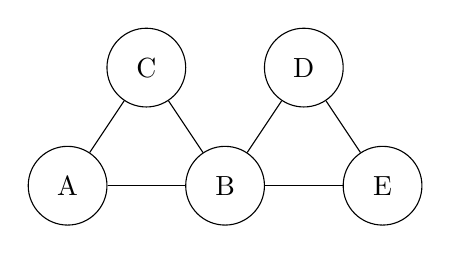
\begin{tikzpicture}[scale=1, every node/.style={draw, circle, minimum size=1cm}]
							\node (A) at (0,0) {A};
							\node (B) at (2,0) {B};
							\node (C) at (1,1.5) {C};
							\node (D) at (3,1.5) {D};
							\node (E) at (4,0) {E};

							\draw (A) -- (B);
							\draw (A) -- (C);
							\draw (B) -- (C);
							\draw (B) -- (D);
							\draw (B) -- (E);
							\draw (D) -- (E);
						\end{tikzpicture}
					\end{center}

				\item \textbf{Grafo dirigido (dígrafo)}: En un grafo dirigido, cada arista tiene una dirección, por lo que $(u, v) \in E$ no implica necesariamente que $(v, u) \in E$ pero tampoco lo prohíbe. Dado este escenario, diremos que \textbf{$u$ se dirige a $v$}.

					\begin{center}
						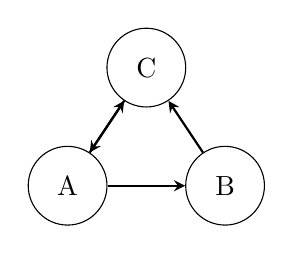
\begin{tikzpicture}[scale=1, every node/.style={draw, circle, minimum size=1cm}, >=stealth]
							\node (A) at (0,0) {A};
							\node (B) at (2,0) {B};
							\node (C) at (1,1.5) {C};

							\draw[->, thick] (A) -- (B);
							\draw[->, thick] (B) -- (C);
							\draw[->, thick] (C) -- (A);
							\draw[->, thick] (A) -- (C);
						\end{tikzpicture}
					\end{center}
				\item \textbf{Grafo ponderado}: Un grafo es ponderado si a cada arista $(u, v) \in E$ se le asigna un peso $w(u, v) \in \mathbb{R}$ que representa costos, distancias, o cualquier otra métrica relevante. Un grafo puede ser ponderado a la vez que dirigido o no dirigido.
					\begin{center}
					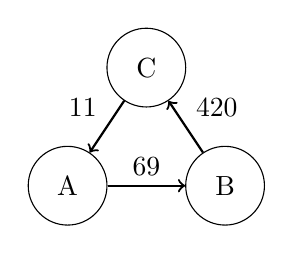
\begin{tikzpicture}[scale=1,
						vertex/.style={draw, circle, minimum size=1cm}
						]
						% Definición de vértices
						\node[vertex] (A) at (0,0) {A};
						\node[vertex] (B) at (2,0) {B};
						\node[vertex] (C) at (1,1.5) {C};

						% Aristas con etiquetas; se anula el estilo global para estos nodos
						\draw[->, thick] (A) -- node[above, draw=none, fill=none] {69} (B);
						\draw[->, thick] (B) -- node[above right, draw=none, fill=none] {420} (C);
						\draw[->, thick] (C) -- node[above left, draw=none, fill=none] {11} (A);
					\end{tikzpicture}
				\end{center}

			\end{itemize}

		\subsection{Propiedades fundamentales de los grafos}
			Los grafos poseen diversas propiedades matemáticas que permiten su análisis estructural.
			Algunas que son especialmente valiosas para el presente estudio son conceptos como la \textit{conectividad}, que nos permite mesurar la importancia que tiene un nodo con respecto a los demás; así también los \textit{caminos}, que nos permiten representar trayectorias; entre otros conceptos.

			\subsubsection{Subgrafos}

			Un subgrafo $H = (V_H, E_H)$ de un grafo $G = (V, E)$ es un grafo tal que $V_H \subseteq V$ y $E_H \subseteq E$.
			Es decir, un subgrafo es una parte de un grafo que mantiene la estructura de nodos y aristas del grafo original.

			Muchos conceptos en la teoría de grafos pueden describirse en términos de subgrafos.

			\subsubsection{Caminos}

			Un \textbf{camino} en un grafo $G$ es un subgrafo en el que los vértices están conectados por una secuencia de aristas sin repeticiones:
			\begin{equation}
				P_k = (v_1, v_2, \dots, v_k) \quad \text{donde } \{v_i, v_{i+1}\} \in E, \forall i \in \{1, \dots, k-1\}.
			\end{equation}

			Los caminos son fundamentales en redes, pues permiten analizar rutas eficientes y la conectividad entre distintos puntos.

			\subsubsection{Ciclos}

			Un \textbf{ciclo} es un camino en el que el primer y el último vértice son el mismo:
			\begin{equation}
				C_k = (v_1, v_2, \dots, v_k, v_1) \quad \text{donde } \{v_k, v_1\} \in E.
			\end{equation}

			Los ciclos en redes ayudan a identificar redundancias estructurales y evaluar posibles congestiones en ciertas áreas.

			\begin{figure}[ht]
				\centering
				\begin{subfigure}{0.3\textwidth}
					\centering
					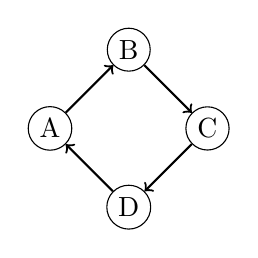
\begin{tikzpicture}[scale=1, every node/.style={circle, draw, fill=white, inner sep=2pt}]
						\node (a) at (0,0) {A};
						\node (b) at (1,1) {B};
						\node (c) at (2,0) {C};
						\node (d) at (1,-1) {D};
						\draw[->, thick] (a) -> (b);
						\draw[->, thick] (b) -> (c);
						\draw[->, thick] (c) -> (d);
						\draw[->, thick] (d) -> (a);
					\end{tikzpicture}
					\caption{Subgrafo}
				\end{subfigure}
				\begin{subfigure}{0.3\textwidth}
					\centering
					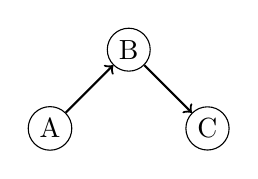
\begin{tikzpicture}[scale=1, every node/.style={circle, draw, fill=white, inner sep=2pt}]
						\node (a) at (0,0) {A};
						\node (b) at (1,1) {B};
						\node (c) at (2,0) {C};
						\draw[->, thick] (a) -> (b);
						\draw[->, thick] (b) -> (c);
					\end{tikzpicture}
					\caption{Camino}
				\end{subfigure}
				\begin{subfigure}{0.3\textwidth}
					\centering
					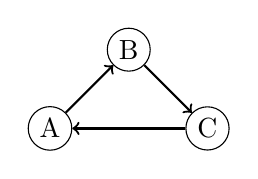
\begin{tikzpicture}[scale=1, every node/.style={circle, draw, fill=white, inner sep=2pt}]
						\node (a) at (0,0) {A};
						\node (b) at (1,1) {B};
						\node (c) at (2,0) {C};
						\draw[->, thick] (a) -> (b);
						\draw[->, thick] (b) -> (c);
						\draw[->, thick] (c) -> (a);
					\end{tikzpicture}
					\caption{Ciclo}
				\end{subfigure}
				\caption{Ejemplos de subgrafo, camino y ciclo en un grafo.}
			\end{figure}

			\subsubsection{Matriz de Adyacencia}
				La matriz de adyacencia es una representación matricial que codifica la estructura de un grafo. Dado un grafo $G=(V,E)$ con $N$ nodos, se define una matriz $A \in \mathbb{R}^{N \times N}$, donde cada elemento $a_{ij}$ indica si existe una conexión directa entre el nodo $i$ y el nodo $j$. En un grafo no ponderado, se establece que:
				\begin{equation}
					a_{ij} =
					\begin{cases}
						1, & \text{si existe una arista entre } i \text{ y } j,\\
						0, & \text{en caso contrario.}
					\end{cases}
				\end{equation}
				En grafos ponderados, cada $a_{ij}$ toma el valor del peso asignado a la conexión, lo que permite cuantificar la intensidad o costo de dicha relación.

		\subsection{Propiedades estructurales}

		Entre las propiedades clásicas que describen la forma en que los vértices se relacionan destacan:
		\begin{itemize}
			\item \textbf{Conectividad}: existe al menos un camino entre cada par de vértices; de lo contrario la red se fragmenta en componentes conexas.
			\item \textbf{Árbol}: grafo conexo sin ciclos. Satisface $|E|=|V|-1$.
			\item \textbf{Diámetro}: longitud del camino más largo entre los caminos más cortos de todos los pares $(u,v)$.
			\item \textbf{Nodo articulación} e \textbf{istmo}: suprimirlos incrementa el número de componentes, evidencia fragilidad local. (Rodrigues, 2013).
			\item \textbf{Número de ciclos independientes}: $\mu = |E|-|V|+p$, donde $p$ es el número de componentes.
		\end{itemize}

		\subsubsection*{Nivel de red}

		\begin{description}

		\item[Índice $\beta$ (conectividad).]
		Mide cuántas aristas existen respecto al número de nodos, es decir, cuántas conexiones “promedio” puede esperar cada vértice. Valores cercanos a $1$ indican una topología arborescente (pocas alternativas de ruta), mientras que valores crecientes reflejan una mayor interconexión y, por tanto, más opciones de recorrido.
		\begin{center}
		$\displaystyle \beta \;=\; \frac{|E|}{|V|}$
		\end{center}

		\item[Índice $\alpha$ (redundancia).]
		Cuantifica la proporción de ciclos efectivamente presentes frente al máximo posible en un grafo planar. Sirve para valorar la resiliencia de la red: cuanto más alto, más caminos alternativos existen ante fallos o congestión. El parámetro $p$ indica el número de componentes conexas (en la práctica, $p=1$ si la red está totalmente conectada).
		\begin{center}
		$\displaystyle \alpha \;=\; \frac{|E| - |V| + p}{\,2|V| - 5\,}$
		\end{center}

		\item[Índice $\gamma$ (densidad planar).]
		Expresa la fracción de aristas observadas con respecto al límite superior para un grafo planar simple ($3|V|-6$). Un $\gamma$ cercano a $1$ denota que la red se aproxima a la máxima densidad planar, mientras que valores bajos sugieren poca malla y mayor fragilidad estructural.
		\begin{center}
		$\displaystyle \gamma \;=\; \frac{|E|}{\,3|V| - 6\,}$
		\end{center}

		\item[Longitud total.]
		Es la suma de las longitudes físicas de todas las aristas—por ejemplo, la distancia vial o la duración promedio del trayecto—y constituye un indicador agregado de la inversión material o de la “extensión” operativa de la red.
		\begin{center}
		$\displaystyle L(G) \;=\; \sum_{(i,j)\in E} \ell_{ij}$
		\end{center}

		\item[Índice de rodeo ($DI$).]
		Compara la distancia efectiva que un viajero debe recorrer dentro de la red ($D_S$) con la distancia euclidiana ($D_T$) entre origen y destino. Valores mayores que $1$ revelan desvíos importantes (trayectorias poco rectas), mientras que valores cercanos a $1$ implican rutas casi directas.
		\begin{center}
		$\displaystyle DI \;=\; \frac{D_S}{D_T}$
		\end{center}

		\item[Brecha espectral ($\Delta$).]
		Se define como la diferencia entre el mayor y el segundo mayor autovalor del operador de transición (o del Laplaciano normalizado). Una brecha grande suele asociarse con redes más “cohesivas” y con tiempos de mezcla rápidos para procesos de difusión (p.\,ej.\,reparto de pasajeros).
		\begin{center}
		$\displaystyle \Delta \;=\; \lambda_{1} - \lambda_{2}$
		\end{center}

		\end{description}

		\subsubsection*{Nivel de nodo}

		\begin{description}

		\item[Grado ($deg$).]
		Cuenta el número de aristas incidentes en un vértice. En redes dirigidas se distingue entre grado de entrada ($deg^{-}$) y grado de salida ($deg^{+}$); su suma refleja la importancia local del nodo como punto de transferencia.
		\begin{center}
		$\displaystyle deg(v) \;=\; deg^{-}(v) + deg^{+}(v)$
		\end{center}

		\item[Centralidad de cercanía ($C_c$).]
		Evalúa qué tan “cerca” se encuentra un nodo de todos los demás en términos de la distancia sobre la red. Un valor elevado (distancias promedio bajas) indica accesibilidad global, útil para ubicar terminales o centros de transbordo.
		\begin{center}
		$\displaystyle C_c(v) \;=\; \frac{1}{\sum_{u\in V} d(u,v)}$
		\end{center}

		\item[Centralidad de intermediación ($C_b$).]
		Mide la proporción de rutas geodésicas (más cortas) entre pares de nodos que pasan por $v$. Detecta “puentes” críticos cuyo fallo incrementaría fuertemente la longitud de los recorridos o desconectaría sectores.
		\begin{center}
		$\displaystyle C_b(v) \;=\; \sum_{s\neq v\neq t}\frac{\sigma_{st}(v)}{\sigma_{st}}$
		\end{center}

		\item[Eccentricidad ($e$).]
		Es la mayor distancia desde $v$ hacia cualquier otro nodo. Representa el “peor caso” de accesibilidad individual; nodos con baja eccentricidad pueden considerarse geográficamente estratégicos dentro de la red.
		\begin{center}
		$\displaystyle e(v) \;=\; \max_{u\in V} d(u,v)$
		\end{center}

		\end{description}

		En conjunto, estos indicadores permiten diagnosticar fortalezas y debilidades tanto globales como locales, fundamentando decisiones sobre expansión, mantenimiento y robustecimiento de la infraestructura de transporte (Rodrigues, 2013).


		\subsection{Vulnerabilidad y resiliencia}

		Para cuantificar la sensibilidad de la red ante fallos se emplea la \emph{eficiencia global}
		\begin{equation}
			E(G)=\frac{1}{N(N-1)}\sum_{i\neq j}\frac{1}{d_{ij}}.
		\end{equation}
		La eliminación de un conjunto crítico $H$ reduce la eficiencia a $E(G\setminus H)$ y la \textbf{vulnerabilidad} se define como
		\begin{equation}
			V=\frac{E(G)-E(G\setminus H)}{E(G)}.
		\end{equation}
		Valores altos de $V$ implican que pocos nodos o aristas concentran la mayor parte del flujo: la red es frágil (Rodrigues, 2013).

		\subsection{Algoritmos fundamentales en teoría de grafos}
			Los algoritmos en teoría de grafos permiten resolver problemas fundamentales como la determinación de caminos más cortos entre nodos. En esta sección, se presentan dos algoritmos esenciales para este propósito: Dijkstra y Floyd-Warshall.

			\subsubsection{Algoritmo de Dijkstra}

			El algoritmo de Dijkstra encuentra el camino más corto desde un nodo fuente $s$ hacia todos los demás nodos en un grafo ponderado con pesos no negativos. Se basa en una estrategia voraz que mantiene un conjunto de nodos visitados y actualiza iterativamente las distancias más cortas conocidas.

			\textbf{Entrada:}
			\begin{itemize}
				\item Un grafo dirigido o no dirigido $G = (V, E)$ con pesos no negativos $w: E \to \mathbb{R}^+$.
				\item Un nodo fuente $s \in V$.
			\end{itemize}

			\textbf{Salida:}
			\begin{itemize}
				\item Distancias mínimas $d(v)$ desde $s$ hacia cada nodo $v \in V$.
				\item Árbol de caminos más cortos.
			\end{itemize}

			\textbf{Procedimiento:}
			\begin{enumerate}
				\item Inicializar $d(s) = 0$ y $d(v) = \infty$ para todos los $v \neq s$.
				\item Crear un conjunto de nodos visitados $S = \emptyset$.
				\item Mientras $S \neq V$:
				\begin{enumerate}
					\item Seleccionar el nodo $u \notin S$ con la menor distancia $d(u)$.
					\item Agregar $u$ a $S$.
					\item Para cada vecino $v$ de $u$ tal que $(u,v) \in E$:
					\begin{itemize}
						\item Si $d(u) + w(u,v) < d(v)$, actualizar $d(v) = d(u) + w(u,v)$.
					\end{itemize}
				\end{enumerate}
			\end{enumerate}

			\subsubsection{Algoritmo de Floyd-Warshall}

			El algoritmo de Floyd-Warshall encuentra el camino más corto entre todos los pares de nodos en un grafo ponderado con pesos arbitrarios (incluyendo negativoss). Se basa en la programación dinámica y mejora iterativamente una matriz de distancias.

			\textbf{Entrada:}
			\begin{itemize}
				\item Un grafo dirigido $G = (V, E)$ con una matriz de pesos $W$.
			\end{itemize}

			\textbf{Salida:}
			\begin{itemize}
				\item Una matriz $D$ donde $D[i][j]$ representa la distancia más corta entre los nodos $i$ y $j$.
			\end{itemize}

			\textbf{Procedimiento:}
			\begin{enumerate}
				\item Inicializar $D$ como la matriz de adyacencia $W$, donde $D[i][j] = w(i,j)$ si existe una arista $(i,j)$, y $\infty$ en caso contrario.
				\item Para cada nodo intermedio $k \in V$:
				\begin{enumerate}
					\item Para cada par de nodos $i, j \in V$:
					\begin{itemize}
						\item Si $D[i][k] + D[k][j] < D[i][j]$, actualizar $D[i][j] = D[i][k] + D[k][j]$.
					\end{itemize}
				\end{enumerate}
			\end{enumerate}

    \section{General Transit Feed Specification (GTFS)}

		El General Transit Feed Specification (GTFS) es un estándar utilizado a nivel internacional para la publicación y análisis de datos sobre el transporte público (GTFS, 2025). Su importancia radica en la posibilidad de modelar la red de transporte mediante datos estructurados que incluyen información sobre agencias, rutas, viajes, horarios, paradas y frecuencias.

		El GTFS permite estructurar información clave sobre el transporte público, facilitando el análisis y la planificación urbana. Sus principales componentes incluyen archivos como \texttt{agency.txt}, \texttt{stops.txt}, \texttt{routes.txt}, \texttt{trips.txt}, \texttt{stop\_times.txt}, \texttt{calendar.txt}, \texttt{frequencies.txt}, \texttt{shapes.txt}, \texttt{fare\_attributes.txt}, \texttt{fare\_rules.txt}, \texttt{transfers.txt} y \texttt{feed\_info.txt}. Estos archivos contienen información sobre operadores de transporte, ubicaciones de paradas, rutas, horarios programados, tarifas y reglas de transbordo. Gracias a su estructura, el GTFS permite integrar sistemas de pago, optimizar la gestión de tarifas y mejorar la accesibilidad a la información de transporte.

		\subsection{Archivos del GTFS}

		A continuación, se presenta una tabla con los archivos incluidos en el GTFS y su descripción:

		\begin{table}[h]
			\centering
			\begin{tabular}{|l|p{10cm}|}
				\hline
				\textbf{Archivo} & \textbf{Descripción} \\
				\hline
				agency.txt & Contiene información sobre las agencias de transporte público. \\
				stops.txt & Define las ubicaciones de paradas y estaciones. \\
				routes.txt & Describe las rutas del servicio de transporte. \\
				trips.txt & Lista los viajes individuales para cada ruta. \\
				stop\_times.txt & Indica los tiempos de llegada y salida en cada parada. \\
				calendar.txt & Define los días de operación del servicio de transporte. \\
				calendar\_dates.txt & Permite definir excepciones a los horarios del calendario. \\
				fare\_attributes.txt & Contiene información sobre tarifas de viaje. \\
				fare\_rules.txt & Especifica reglas sobre la aplicación de tarifas. \\
				shapes.txt & Describe las formas geométricas de las rutas. \\
				frequencies.txt & Define los intervalos entre viajes en rutas con horarios de frecuencia fija. \\
				transfers.txt & Especifica las reglas de transferencia entre rutas. \\
				feed\_info.txt & Contiene metadatos sobre el conjunto de datos del GTFS. \\
				pathways.txt & Define conexiones peatonales dentro de estaciones. \\
				levels.txt & Especifica los diferentes niveles dentro de estaciones. \\
				location\_groups.txt & Agrupa varias ubicaciones relacionadas en el sistema de transporte. \\
				attributions.txt & Contiene información sobre atribuciones y derechos de los datos. \\
				translations.txt & Define traducciones de los valores mostrados al usuario. \\

				\hline
			\end{tabular}
			\caption{Archivos del GTFS y su descripción.}
			\label{tab:gtfs_files}
		\end{table}

		La adopción del GTFS ha sido clave en diversas ciudades para mejorar la planificación y operación del transporte público. Además, en muchas otras ciudades, su implementación ha facilitado la integración de múltiples operadores en una única plataforma de información, permitiendo la interoperabilidad de diferentes servicios de transporte y promoviendo la movilidad sostenible.

	\section{Casos de aplicación}
		\subsection{Sydney}
		\label{sec:sydney}

		Un primer ejemplo en el uso de la teoría de grafos en el estudio del transporte público, es el de Sydney con el estudio de Zhao \textit{et al.} sobre la estimación de matrices origen–destino (OD) a escala de parada en el corredor noroeste, específicamente a lo largo de la autopista M2.

		El corredor M2 abarca varios \textit{Statistical Areas Level 2} (SA2) en la periferia norte-occidental de Sídney y concentra:
		\begin{itemize}
		  \item 76 rutas de autobús,
		  \item 2 líneas ferroviarias suburbanas,
		  \item 1 línea de metro,
		  \item 3 799 paradas de autobús y 7 estaciones ferroviarias/metro.
		\end{itemize}
		La alta densidad de infraestructura y la combinación de modos convierten a esta zona en un laboratorio idóneo para evaluar técnicas de estimación OD de alta resolución.

		\begin{enumerate}
		  \item \textbf{Demanda.} Registros de \emph{smart card} correspondientes a junio de 2017, filtrados para eliminar anomalías y agregados en intervalos de 15 min. El análisis se centró en la hora punta matutina (7:00–11:00).
		  \item \textbf{Oferta.} Datos GTFS históricos (OpenData NSW y TransitFeeds) que proporcionan recorridos, horarios y distancias programadas.
		  \item \textbf{Métricas topológicas.} A partir del GTFS se derivaron indicadores de conexión, cercanía y rectitud, insumos clave para el cálculo de costos generalizados.
		\end{enumerate}

		El procedimiento se desarrolla en cinco pasos principales:
		\begin{enumerate}
		  \item \textbf{Vector GA.} Cálculo de generación (\textit{tap-ons}) y atracción (\textit{tap-offs}) por parada.
		  \item \textbf{Modelo gravitacional.} Variante doblemente restringida con tres funciones de disuasión (potencia, exponencial y Tanner).
		  \item \textbf{Escenarios de calibración.}
				\begin{itemize}
				  \item S1 – \emph{Traverse search} con un único costo.
				  \item S2 – Algoritmo de Hyman con combinaciones de costos simples y fusionados.
				  \item S3 – Ponderación entrópica aplicada a costos fusionados.
				\end{itemize}
		  \item \textbf{Costos generalizados.} Se probaron seis atributos (distancia, tiempo, tarifa, conexión, cercanía, rectitud) y sus combinaciones. La ponderación entrópica asigna mayor peso a los atributos más informativos y estables.
		  \item \textbf{Criterio de convergencia.} Diferencia $<0.01\%$ entre generación-atracción observada y estimada, con un máximo de 20 iteraciones.
		\end{enumerate}

		\paragraph{Red de autobuses.}
		El escenario S3E2 —ponderación entrópica con la combinación \emph{cercanía + rectitud}— registró el mejor desempeño: redujo el MAE en 5 \% y el RMSE en 4 \% frente a la mejor configuración de S2, con un tiempo de cómputo 40 \% menor. El MAPE horario se mantuvo por debajo del 35 \%, salvo un repunte entre 8:30 y 9:30 que coincide con el pico de demanda. Aunque la búsqueda exhaustiva (S1) alcanzó precisiones ligeramente superiores (error ≈ 6.4 \%), el costo computacional fue prohibitivo (más de dos horas).

		\paragraph{Red ferroviaria y de metro.}
		Dada la menor complejidad de la red, un costo único basado en el tiempo de viaje (S2E1) bastó para alcanzar un MAPE mínimo. Sin embargo, la misma combinación \emph{cercanía + rectitud} ponderada entrópicamente (S3E2) suavizó los errores extremos (RMSE –23 \%) y mejoró la precisión media un 19 \%, todo ello con tiempos de cómputo inferiores a un segundo.

		Los resultados muestran que las métricas topológicas puras (cercanía y rectitud) capturan eficazmente la fricción espacial percibida por los usuarios en redes de autobuses extensas y ramificadas. La ponderación entrópica evita sobre-parametrizar el modelo y acelera la convergencia, lo cual es esencial cuando se realizan iteraciones finas por intervalo temporal. En redes más compactas, donde el tiempo de viaje está más estandarizado, este atributo recupera protagonismo.

		\paragraph{Resultados y conclusiones}
		Los resultados muestran que las métricas topológicas puras (cercanía y rectitud) capturan eficazmente la fricción espacial percibida por los usuarios en redes de autobuses extensas y ramificadas. La ponderación entrópica evita sobre-parametrizar el modelo y acelera la convergencia, lo cual es esencial cuando se realizan iteraciones finas por intervalo temporal. En redes más compactas, donde el tiempo de viaje está más estandarizado, este atributo recupera protagonismo.
		\bigskip

		La inclusión de costos topológicos ponderados entrópicamente en un modelo gravitacional mejora simultáneamente la precisión y la eficiencia computacional en la estimación OD a nivel de parada. El corredor M2 demuestra que una adecuada selección-ponderación de atributos puede reducir los errores promedio en más del 20\% sin incurrir en tiempos de cálculo excesivos, aportando lecciones metodológicas valiosas para los casos de Resistencia y Guadalajara.

		\subsection{Resistencia}

		El presente apartado resume el artículo de Cardozo, Gómez y Parras (2009), que aplica Teoría de Grafos y SIG al micro-centro de Resistencia, Chaco (≈ 100 ha). Su objetivo es describir la estructura y accesibilidad de la red de autobuses urbanos para, más adelante, contrastarla con los casos de Sydney y Guadalajara.

		El área de estudio abarca el casco céntrico delimitado por las avenidas Moreno, Rodríguez Peña, Belgrano, Wilde, Rivadavia, Paraguay, San Martín e Italia. La red simplificada consta de \textbf{48 nodos (paradas agregadas)} y \textbf{61 arcos (tramos de ruta)}.

		\begin{enumerate}
		  \item \textbf{Infraestructura.} Relevamiento GPS (Parras 2008) de paradas y recorridos, georreferenciado sobre cartografía vial municipal 2007.
		  \item \textbf{Modelos SIG.} Construcción de grafo, matrices de conectividad y accesibilidad; estimación de densidades \emph{kernel} con radio 200 m y píxel 5 m para visualizar la oferta.
		\end{enumerate}

		\begin{enumerate}
		  \item \textbf{Conectividad global.} Índices $\beta$, $\mu$ (número ciclomático) y $\alpha$.
		  \item \textbf{Accesibilidad nodal.} Número Asociado (NS) y Shimbel derivados de la matriz de accesibilidad topológica.
		  \item \textbf{Accesibilidad global.} Índice $G$ y Accesibilidad Media (IAM $=G/n$).
		  \item \textbf{Visualización espacial.} Mapas de suma de conexiones, NS, Shimbel e intensidad \emph{kernel}.
		\end{enumerate}

		\paragraph{Conectividad.}
		El grafo exhibe $\beta = 1.27$, indicando una red compleja; sólo el 11.3\% de la conectividad máxima teórica se ha materializado. Presenta $\mu = 14$ circuitos y $\alpha = 0.154$, es decir, un 15\% del máximo posible de circuitos.

		\paragraph{Centralidad.}
		El nodo 23 (Julio A. Roca × Santa María de Oro) alcanza el \emph{grado 5}; siete nodos más poseen grado 4. En contraste, los nodos 1, 41 y 48 (extremos de red) sólo tienen una conexión.

		\paragraph{Accesibilidad.}
		El análisis NS–Shimbel revela un claro gradiente centro-periferia: los valores mínimos se concentran alrededor de la Plaza 25 de Mayo, incrementándose hacia los límites norte y este. Los indicadores globales son $G = 11\,564$ y $\mathrm{IAM}=241$ arcos; por debajo de ese umbral se agrupan los nodos centrales.

		\paragraph{Distribución espacial.}
		El mapa de densidad \emph{kernel} ponderado por grado muestra un “pico” Centro-Oeste alineado con la calle J. D. Perón; la densidad se diluye hacia el Este y Noroeste, mientras que un corredor intermedio emerge en el Sudeste a lo largo de Av. 9 de Julio.

		\paragraph{Resultados y conclusiones.}
		La red céntrica de Resistencia concentra paradas y conexiones en torno a la plaza principal y ejes comerciales, creando fuertes desequilibrios de accesibilidad. El bajo porcentaje de conectividad materializada (11 \%) y el IAM relativamente alto evidencian oportunidades para redistribuir servicios hacia la periferia y reducir dependencias radiales. Las visualizaciones \emph{kernel} refuerzan la necesidad de políticas que diversifiquen la oferta fuera del Centro-Oeste.

		\bigskip

		El uso combinado de índices topológicos e instrumentos SIG permitió diagnosticar una \emph{sobrecarga central} y una \emph{periferia subatendida}. Las métricas globales y nodales servirán de referencia comparativa con Guadalajara y como línea base para evaluar intervenciones que busquen equilibrar la accesibilidad en la red urbana chaqueña.

	\subsection{Guadalajara}
		\label{sec:guadalajara}

		\subsubsection*{Fuente y alcance del estudio}
		Esta sección expone con mayor detalle la metodología y los resultados de Barraza y Estrada (2021), quienes evaluaron una red de transporte \emph{alternativa} para la Zona Metropolitana de Guadalajara (ZMG). El análisis se centra en tres dimensiones estructurales: (i) eficiencia temporal (\textit{grade of accessibility}), (ii) fricción espacial (\textit{Deuter index}) y (iii) resiliencia/vulnerabilidad (\textit{hub dependence}).

		\subsubsection*{Preparación de datos}
		\begin{enumerate}
		  \item \textbf{Zonificación hexagonal.} Se tessela el área de servicio (≈ 330 km$^{2}$) con 398 hexágonos de apotema 670 m; los centroides son los nodos OD.
		  \item \textbf{Creación de GTFS sintético.} La red propuesta (2033 paradas, 39 rutas ortogonales) se codifica como feed GTFS; se identifican modos, secuencias y tiempos de viaje.
		  \item \textbf{Generación de matriz $N\times N$ con \texttt{OpenTripPlanner} (OTP).}
				\begin{compactitem}
				  \item Configurar OTP con la malla vial de OSM y el GTFS.
				  \item Solicitar viajes entre todos los centroides (≈ 158 k queries).
				  \item Exportar un \texttt{data frame} con tiempos parciales (caminar, espera, vehículo) y distancias.
				\end{compactitem}
		  \item \textbf{Transformación a grafo \texttt{igraph}.} Agrupar paradas contiguas, eliminar aisladas y calcular enlaces con sus tiempos; resultado: grafo dirigido ponderado con 2033 vértices y 4704 aristas.
		\end{enumerate}

		\subsubsection*{Paso 1 – Accesibilidad (Índice de Shimbel)}
		\paragraph{Definición.} Para cada nodo $x$ se computa
		\[
		C(x)=\frac{1}{N-1}\sum_{y=1}^{N} d(x,y),
		\]
		donde $d(x,y)$ es el tiempo de viaje mínimo entre $x$ e $y$. Un valor bajo implica mayor accesibilidad.

		\paragraph{Resultados.}
		\begin{itemize}
		  \item \textit{Tiempo medio de viaje global}: 70 min (52 vehículo + 12 caminar + 6 espera).
		  \item \textit{Shimbel global}: 0.015.
		  \item \textit{Distribución nodal}: 46–115 min; el 75 % de los pares OD están por debajo de 70 min.
		\end{itemize}

		\paragraph{Interpretación.} La geometría ortogonal y la velocidad comercial ($\bar v=22$ km/h) concentran la accesibilidad en los cruces Calzada–Lázaro Cárdenas y el Centro Histórico.

		\subsubsection*{Paso 2 – Fricción espacial (Índice de Deuter)}
		\paragraph{Definición.}
		\[
		DI=\frac{D_S}{D_T},
		\]
		donde $D_S$ es la distancia euclídea y $D_T$ la distancia real sobre la red. $DI\!\to\!1$ implica trayectos casi rectilíneos.

		\paragraph{Resultados.} $DI=0.63$ con $D_T=18.81$ km y $D_S=11.91$ km. El 75 % de los viajes recorren menos de 25 km sobre la red, frente a menos de 15 km en línea recta.

		\paragraph{Interpretación.} El trazado ortogonal reduce rodeos, pero la necesidad de un trasbordo medio mantiene la fricción por encima del ideal.

		\subsubsection*{Paso 3 – Resiliencia y vulnerabilidad (Dependencia de \textit{hubs})}
		\begin{enumerate}[label=\alph*)]
		\item \textbf{Betweenness centrality}
			  \[
			  C_B(i)=\sum_{j<k}\frac{\sigma_{jk}(i)}{\sigma_{jk}},
			  \]
			  con $\sigma_{jk}$ caminos mínimos entre $j$ y $k$.
			  \begin{compactitem}
				\item Máx.: 746 551, Prom.: 65 824, Min.: 0.
				\item Tres super-nodos (Centro, Calzada, Periférico Sur) concentran más del 40 % del flujo óptimo.
			  \end{compactitem}

		\item \textbf{Central Point Dominance (CPD)}
			  \[
			  C_B^{\ast}=\frac{1}{n-1}\sum_{i}(B_{\max}-B_i)=680\,726.
			  \]
			  Valor alto $\Rightarrow$ fuerte polarización.

		\item \textbf{Longitud de camino medio (APL)} normal: 36.27 paradas.
			  \begin{compactitem}
				\item Remoción aleatoria 15 % nodos → APL = 46 ( + 27 %; 89 min).
				\item Remoción dirigida (top 10 % betweenness) → APL = 69 ( + 91 %; 133 min).
			  \end{compactitem}

		\item \textbf{Spectral gap} $\Delta\lambda=0.155$ indica baja expansividad y susceptibilidad a cortes críticos.
		\end{enumerate}

		\paragraph{Interpretación.}
		La red es robusta a fallas dispersas pero extremadamente frágil frente a interrupciones en sus tres super-nodos. La jerarquía betweenness–CPD explica la sensibilidad: duplicar conexiones periféricas o añadir diagonales disminuiría $\Delta\lambda$ y CPD, amortiguando el efecto de fallas locales.

		\subsubsection*{Conclusiones para Guadalajara}
		La red alternativa ofrece \textit{buenos tiempos medios} y \textit{rodeos contenidos}; no obstante, su dependencia de pocos hubs la deja expuesta a fallas estratégicas. Reforzar cruces secundarios, introducir rutas diagonales y balancear frecuencias mitigaría la polarización sin sacrificar la eficiencia obtenida en los pasos 1 y 2.

		%--- Fin sección Guadalajara ---

\chapter{Análisis territorial de la Zona Metropolitana de Guadalajara}
	Dentro del contexto de los métodos cuantitativos creados para analizar las redes de transporte público, existe una constante preocupación de ser "guíados a una perspectiva mecanicista donde la correspondencia con la realidad se vuelve algo secundario" (Rodrigues, 2013). En este sentido, una de las necesidades de estos métodos es la de tener una perspectiva multidisciplinar que integre teorías de otros campos que le den un sentido a cualquier resultado obtenido por métodos cuantitativos.

	Una de estas disciplinas a tener en cuenta es el urbanismo, que provee de un entendimiento de la geografía del terreno, su división político-administrativa, las jerarquías funcionales de sus equipamientos y la dinámica de usos de suelo que, en conjunto, moldean la morfología urbana; de esta manera, los indicadores cuantitativos dejan de ser meras abstracciones numéricas y se reinterpretan como huellas cuantificables de procesos históricos, sociales y económicos que han dado forma —y siguen condicionando— la movilidad cotidiana.

	Cuando hablamos de la Zona Metropolitana de Guadalajara (ZMG), diversos organismos públicos y privados han realizado esfuerzos significativos para comprender su dinámica urbana desde distintas perspectivas. En este capítulo abordaremos específicamente el trabajo del Instituto Metropolitano de Planeación (IMEPLAN), organismo encargado de «diseñar, gestionar e impulsar herramientas para el crecimiento integral de la ciudad desde un enfoque sustentable y resiliente» (IMEPLAN, 2023).

	En primer lugar, analizaremos su Plan de Ordenamiento Territorial, que ofrece una descripción detallada de la geografía de la ZMG, la distribución espacial de diversos indicadores urbanos relevantes y una zonificación específica. Esta información será clave para contextualizar e interpretar los resultados de nuestro análisis.

	Posteriormente, revisaremos cómo IMEPLAN, sobre la base del ordenamiento territorial ya mencionado, ha abordado la movilidad ciudadana en la ZMG. Este análisis aporta una herramienta particularmente útil para nuestro estudio: las líneas del deseo, que ilustran los orígenes y destinos más frecuentes de los desplazamientos cotidianos en la metrópoli. Así, podremos evaluar si la red actual de transporte público cumple efectivamente con su función principal, es decir, conectar de forma adecuada a la ciudadanía con los lugares a los que necesita desplazarse diariamente.

	\section{División territorial de la ZMG}
		En 2016 se publicó el documento \textit{POTmet: plan de ordenamiento territorial metropolitano del AMG} (POTmet, en delante). Dentro de dicho documento el imeplan propone una forma de segmentar a la ZMG basándose en un modelo policéntrico de ciudad que "busca a través de una identificación metódica de las centralidades, contribuir a un mejor equilibrio espacial en el territorio del AMG, mejorando la distribución de equipamiento, la repartición de la población, la administración de las zonas para crecimiento y en general, todo lo que contribuya a fortalecer un sistema de ciudades aún incipiente en el territorio metropolitano" (imeplan, 2016, p. 265). Dichas centralidades permiten una mejor planificación y análisis de la movilidad urbana, facilitando el diseño de estrategias de transporte más eficientes (imeplan, 2016).

			\subsubsection{Definición y delimitación de la ZMG}
				La ZMG está conformada por los municipios de Guadalajara, Zapopan, Tlaquepaque, Tonalá, El Salto, Ixtlahuacán de los Membrillos y Juanacatlán.
				Su delimitación geográfica se encuentra establecida en el Plan de Ordenamiento Territorial Metropolitano (imeplan, 2016).

			\subsubsection{Centralidades}
				En el POTmet se define centralidad de la siguiente manera:
				\begin{center}
					Son unidades urbanas vinculadas por una estructura vial y que desempeñan una función esencial en la dinámica urbana del área metropolitana, definidas esencialmente por su concentración de empleo, población, transporte y prestación de servicios, además se caracterizan por un alto potencial de generación de identidad y arraigo entre sus habitantes.
				\end{center}
				Para delimitar estas centralidades se toman en cuenta aquellas concentraciones urbanas de entre 10,000 y 500,000 habitantes (imeplan, 2016), luego se estiman los siguientes métricos para cada una de ellas:

				\begin{itemize}
					\item \textbf{Productividad}
					\begin{itemize}
						\item Unidades económicas: cantidad de unidades económicas por centralidad.
						\item Personal ocupado: personal ocupado generado por las unidades económicas.
						\item Índice de demanda laboral (promedio): describe la relación entre población residente local y oferta laboral local.
						\item Densidad de población residente: Capas de datos que contienen los valores de densidad de población (personas/ha) por manzanas de la ZMG.
					\end{itemize}

					\item \textbf{Infraestructura}
					\begin{itemize}
						\item Rutas de transporte público: Cantidad de rutas que interceptan con la centralidad.
						\item Capacidad de carga de transporte público: Definida a través del cálculo de flota entre intervalo de las rutas de transporte público que interceptan con la centralidad.
						\item Transporte público masivo: Cantidad de líneas de transporte público masivo que interceptan por centralidad.
					\end{itemize}

					\item \textbf{Calidad de vida}
					\begin{itemize}
						\item Índice de suficiencia de servicios (promedio).
						\item Equipamientos distritales: Proporcionados por los municipios en sus PPDU y clasificados con base en el reglamento estatal de zonificación. Son polígonos de equipamiento de educación, cultura, salud, servicios institucionales y culto que sirven a amplios sectores de los centros de población.
						\item Equipamientos centrales: Proporcionados por los municipios en sus PPDU y clasificados con base en el reglamento estatal de zonificación. Son polígonos de equipamiento que sirven a la totalidad del centro de población.
						\item Equipamientos regionales: Proporcionados por los municipios en sus PPDU y clasificados con base en el reglamento estatal de zonificación. Son polígonos de equipamiento con cobertura de servicio que supera a la ciudad.
					\end{itemize}

					\item \textbf{Otros indicadores}
					\begin{itemize}
						\item Ponderación: Peso relativo de cada centralidad en la evaluación global.
					\end{itemize}
				\end{itemize}

			Una vez se obtienen estas métricas, los datos se normalizan y se otorga un peso a cada centralidad tomando como referencia a la centralidad que mayor puntaje haya obtenido. De este proceso obtenemos la siguiente tabla:

			\begin{table}[H]
			\centering
			\scriptsize
			\setlength{\tabcolsep}{3pt}
			\begin{tabular}{|l|c|c|c|c|c|c|c|c|c|c|}
			\hline
			\textbf{CENTRALIDAD} &
			\begin{tabular}[c]{@{}c@{}}Rutas\\transp.\\público\end{tabular} &
			\begin{tabular}[c]{@{}c@{}}Cap.\\carga\\transp.\end{tabular} &
			\begin{tabular}[c]{@{}c@{}}Dens.\\pobl.\end{tabular} &
			\begin{tabular}[c]{@{}c@{}}Pers.\\ocup.\end{tabular} &
			\begin{tabular}[c]{@{}c@{}}Equip.\end{tabular} &
			\begin{tabular}[c]{@{}c@{}}Línea\\transp.\\masivo\end{tabular} &
			\begin{tabular}[c]{@{}c@{}}Unid.\\econ.\end{tabular} &
			\begin{tabular}[c]{@{}c@{}}Índice\\sufic.\\serv.\end{tabular} &
			\begin{tabular}[c]{@{}c@{}}Índice\\dem.\\lab.\end{tabular} &
			Pond. \\
			\hline
			Centro Guadalajara & 1,00 & 1,00 & 0,40 & 1,00 & 1,00 & 1,00 & 1,00 & 1,00 & 1,00 & 1,00 \\
			Centro Zapopan & 0,52 & 0,20 & 1,00 & 0,52 & 0,76 & 0,50 & 0,42 & 1,00 & 0,38 & 0,82 \\
			Centro Tlaquepaque & 0,69 & 0,32 & 1,00 & 0,48 & 0,94 & 0,50 & 0,58 & 1,00 & 0,21 & 0,82 \\
			Tonalá Centro & 0,37 & 0,21 & 1,00 & 0,52 & 0,13 & 0,00 & 0,66 & 1,00 & 0,27 & 0,74 \\
			Expo-Chapalita & 0,54 & 0,29 & 0,45 & 0,66 & 0,58 & 0,00 & 0,28 & 0,83 & 0,57 & 0,63 \\
			Las Águilas & 0,46 & 0,21 & 1,00 & 0,34 & 0,36 & 0,00 & 0,30 & 1,00 & 0,02 & 0,59 \\
			Oblatos & 0,48 & 0,27 & 1,00 & 0,34 & 0,13 & 0,00 & 0,46 & 1,00 & -0,25 & 0,58 \\
			Miravalle & 0,35 & 0,17 & 1,00 & 0,23 & 0,27 & 0,50 & 0,30 & 1,00 & -0,27 & 0,58 \\
			Parque Solidaridad-Tetlán & 0,31 & 0,20 & 1,00 & 0,21 & 0,00 & 0,50 & 0,34 & 1,00 & -0,36 & 0,52 \\
			Providencia & 0,30 & 0,21 & 0,40 & 0,48 & 0,85 & 0,00 & 0,33 & 0,80 & 0,51 & 0,49 \\
			Centro Sur & 0,28 & 0,15 & 1,00 & 0,25 & 0,31 & 0,50 & 0,12 & 0,58 & 0,13 & 0,49 \\
			Santa Anita & 0,14 & 0,05 & 1,00 & 0,12 & 0,22 & 0,00 & 0,16 & 0,45 & -0,05 & 0,46 \\
			Huentitán & 0,37 & 0,20 & 1,00 & 0,14 & 0,04 & 0,00 & 0,16 & 0,80 & -0,13 & 0,46 \\
			Las Pintitas & 0,37 & 0,04 & 0,52 & 0,25 & 0,40 & 0,00 & 0,33 & 0,41 & -0,09 & 0,43 \\
			Santa Fe & 0,26 & 0,16 & 1,00 & 0,12 & 0,00 & 0,00 & 0,12 & 0,60 & -0,18 & 0,43 \\
			Tlajomulco de Zúñiga & 0,15 & 0,07 & 0,72 & 0,24 & 0,18 & 0,00 & 0,23 & 0,50 & 0,09 & 0,37 \\
			El Salto & 0,06 & 0,02 & 0,75 & 0,12 & 0,58 & 0,00 & 0,17 & 0,60 & -0,01 & 0,37 \\
			San Martín de las Flores & 0,09 & 0,02 & 1,00 & 0,09 & 0,18 & 0,00 & 0,14 & 0,43 & -0,16 & 0,31 \\
			Tesistán & 0,09 & 0,07 & 0,76 & 0,12 & 0,22 & 0,00 & 0,16 & 0,40 & -0,08 & 0,29 \\
			Zapotlanejo & 0,00 & 0,00 & 0,32 & 0,25 & 0,00 & 0,00 & 0,44 & 0,50 & 0,00 & 0,29 \\
			Base Aérea & 0,07 & 0,04 & 0,73 & 0,23 & 0,13 & 0,00 & 0,13 & 0,28 & -0,02 & 0,28 \\
			Toluquilla & 0,26 & 0,16 & 0,47 & 0,18 & 0,18 & 0,00 & 0,06 & 0,28 & 0,04 & 0,28 \\
			San José del Castillo & 0,06 & 0,02 & 0,74 & 0,13 & 0,00 & 0,00 & 0,10 & 0,36 & -0,04 & 0,27 \\
			Coyula & 0,17 & 0,09 & 0,40 & 0,07 & 0,18 & 0,00 & 0,09 & 0,43 & -0,02 & 0,24 \\
			Santa Cruz del Valle & 0,06 & 0,01 & 0,54 & 0,05 & 0,00 & 0,00 & 0,08 & 0,28 & -0,12 & 0,19 \\
			Santa Cruz de las Flores & 0,02 & 0,00 & 0,53 & 0,06 & 0,04 & 0,00 & 0,05 & 0,10 & -0,04 & 0,16 \\
			Ixtlahuacán & 0,00 & 0,00 & 0,38 & 0,04 & 0,00 & 0,00 & 0,07 & 0,20 & -0,03 & 0,15 \\
			\hline
			\end{tabular}
			\caption{Centralidades y sus indicadores}
			\label{tab:centralidades}
			\end{table}

            Para poder analizar la estructura de la red de transporte público, cada una de las centralidades más extensas se dividen en dos, mientras que aquellas centralidades de menos extensión se combinan en una sola (imeplan, 2023). Una vez realizado este procedimiento, nos queamos con las siguientes zonas por cada municipio:

            \begin{table}[H]
            \centering
            \small
            %\rowcolors{1}{white}
            \begin{tabular}{|c|l|l|}
            \hline
            \textbf{Código} & \textbf{Ubicación} & \textbf{Municipio} \\
            \hline
            24A & Bugambilias - Palomar & Tlajomulco de Zúñiga \\
            24B & Las Águilas - Miramar & Zapopan \\
            25 & Santa Ana - El Briseño & Zapopan \\
            26 & La Cantera & Zapopan \\
            29F & La Alcantarilla & El Salto \\
            30 & Santa Anita & Tlajomulco de Zúñiga \\
            30F & Bosques de Santa Anita & Tlajomulco de Zúñiga \\
            32 & Las Liebres & San Pedro Tlaquepaque \\
            34 & Toluquilla & San Pedro Tlaquepaque \\
            35 & Las Pintitas & El Salto \\
            37F & Santa Cruz del Valle & Tlajomulco de Zúñiga \\
            38 & Santa Fe - Chulavista & Tlajomulco de Zúñiga \\
            39F & Lomas del Sur - Hacienda Los Fresnos II & Tlajomulco de Zúñiga \\
            40 & Lázaro Cárdenas del Río & Tonalá \\
            41 & Coyula & Tonalá \\
            42 & Centro Tonalá & Tonalá \\
            43 & Centro Sur - Balcones de Santa María & San Pedro Tlaquepaque \\
            44 & Valdepeñas - Centinela & Zapopan \\
            45 & Tololotlán & Tonalá \\
            46F & Valle de los Molinos - Copalita & Zapopan \\
            48F & Matatlán - La Purísima & Zapotlanejo \\
            49F & La Laja & Zapotlanejo \\
            50 & Santa Fe Zapotlanejo & Zapotlanejo \\
            \hline
            \end{tabular}
            \end{table}

            \begin{table}[H]
            \centering
            \small
            %\rowcolors{1}{white}
            \begin{tabular}{|c|l|l|}
            \hline
            \textbf{Código} & \textbf{Ubicación} & \textbf{Municipio} \\
            \hline
            51F & San Miguel Cuyutlán - San Lucas Evangelista & Tlajomulco de Zúñiga \\
            52 & San José del Castillo & El Salto \\
            53 & Atequiza & Ixtlahuacán de los Membrillos \\
            54 & La Capilla & Ixtlahuacán de los Membrillos \\
            57 & La Gigantera & San Pedro Tlaquepaque \\
            59 & Cajititlán & Tlajomulco de Zúñiga \\
            60 & El Salto & El Salto \\
            61 & Tesistán & Zapopan \\
            63F & La Azucena & Zapopan \\
            65A & El Bajío & Zapopan \\
            65B & Base Aérea & Zapopan \\
            68A & Constitución - Auditorio & Zapopan \\
            68B & Centro Zapopan & Zapopan \\
            69A & Providencia - Minerva & Guadalajara \\
            69B & Puerta de Hierro - Autónoma & Zapopan \\
            70A & San Juan de Dios & Guadalajara \\
            70B & Centro Guadalajara & Guadalajara \\
            Acceso Carretera Vallarta & Acceso Carretera Vallarta & Zapopan \\
            Acceso Carretera Colotlán & Acceso Carretera Colotlán & Zapopan \\
            Acceso Carretera Saltillo & Acceso Carretera Saltillo & Zapopan \\
            Acceso Carretera Zapotlanejo & Acceso Carretera Zapotlanejo & Zapotlanejo \\
            Acceso Carretera Chapala & Acceso Carretera Chapala & Ixtlahuacán de los Membrillos \\
            Acceso Av. López Mateos & Acceso Av. López Mateos & Tlajomulco de Zúñiga \\
            Aeropuerto & Aeropuerto & Tlajomulco de Zúñiga \\
            \hline
            \end{tabular}
            \caption{Puntos de acceso}
            \label{tab:accesos}
            \end{table}

		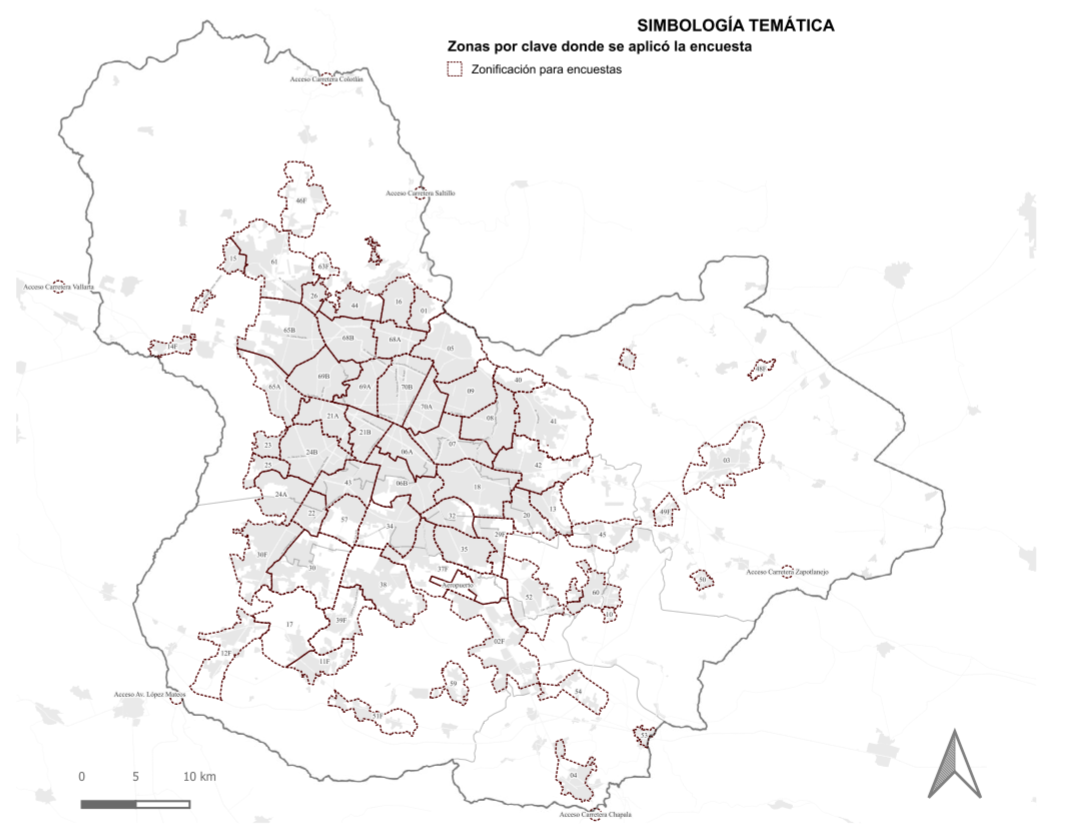
\includegraphics[scale = 0.7]{Zonas_clave_eod.png}



	\section{Encuesta origen-destino 2023}
        El Instituto de Planeación y Gestión del Desarrollo del Área Metropolitana de Guadalajara (Imeplan) realizó la Encuesta Origen Destino 2023 (EOD-2023) con el fin de obtener una herramienta actualizada y eficaz para la planificación de la movilidad. Esta encuesta permite comprender la evolución urbana, identificar tendencias de desplazamiento y determinar las necesidades de infraestructura y servicios para los habitantes de la metrópoli, especialmente en un contexto post-pandemia. La EOD-2023 busca analizar la relación entre la estructura urbana y los patrones de viaje, detectando deficiencias y sirviendo como insumo fundamental para la actualización del Plan Integral de Movilidad Urbana Sustentable (PIMUS) y del Plan de Ordenamiento Territorial Metropolitano (POTmet).

            \subsection{Metodología y alcances}
            La EOD-2023 se llevó a cabo entre marzo y mayo de 2023, con la participación de "Polymetrix Consulting S.A de C.V" para el trabajo de campo y levantamiento de información. El universo de estudio comprendió los 9 municipios que conforman el Área Metropolitana de Guadalajara (AMG): Guadalajara, Zapopan, San Pedro Tlaquepaque, Tlajomulco de Zúñiga, Tonalá, El Salto, Juanacatlán, Ixtlahuacán de los Membrillos y Zapotlanejo.

            Se aplicó un Muestreo Aleatorio Estratificado Trietápico Probabilístico, con un nivel de confianza del 95\% y un margen de error de ±5\% por zona de estudio. El diseño muestral se realizó por zonas, delimitadas con base en las centralidades definidas en el POTmet (2016), donde las centralidades de gran extensión se subdividieron en dos zonas y aquellas de dimensiones mínimas se fusionaron en una sola. Esto se hizo para reflejar la estructura de centralidades y asegurar la disponibilidad de información para caracterizar centralidades con menos población.

            La recolección de información se realizó mediante dos cuestionarios:
            \begin{itemize}
                \item \textbf{Cuestionario de vivienda:} para caracterizar aspectos generales de la vivienda, número de habitantes, ingresos, tenencia de vehículos, problemas de movilidad en la zona, etc.
                \item \textbf{Cuestionario de habitantes:} para determinar las características de los viajes de cada habitante (de 6 años o más), modos y propósitos de los mismos.
            \end{itemize}
            En total, se realizaron encuestas en 17,901 viviendas y a 58,061 residentes.

            Los principales objetivos y alcances de la encuesta fueron:
            \begin{itemize}
                \item Obtener información para caracterizar los viajes cotidianos de los habitantes del AMG.
                \item Determinar el número y motivo de los viajes, modos de transporte empleados, orígenes y destinos, horarios de mayor demanda, gestión del estacionamiento, duración y costo de los viajes.
                \item Identificar patrones de movilidad en términos de género, edad, ocupación, ingreso, lugar de residencia y nivel educativo.
                \item Estimar la cantidad de viajes realizados en el AMG y generar indicadores de movilidad del cuidado.
                \item Conocer los principales problemas de movilidad en general y del transporte público en particular, por zona de estudio.
                \item Servir como insumo para la actualización del PIMUS y del POTmet.
            \end{itemize}
            Una limitación reconocida es la posible omisión de algunos viajes cortos por parte de los encuestados.

            \subsection{Resultados generales}
            La EOD-2023 registró un total de 11,769,386 viajes realizados en un día laborable tipo en el AMG. De estos, el 51.7\% fueron realizados por mujeres y el 48.3\% por hombres.

            En cuanto a la distribución modal general, los tres modos de transporte más utilizados fueron:
            \begin{itemize}
                \item \textbf{Viajes a pie:} 43.2\% del total.
                \item \textbf{Vehículo particular:} 28.1\% del total.
                \item \textbf{Transporte público:} 21.6\% del total.
            \end{itemize}
            Se identificaron tres horarios de máxima demanda de viajes: a las 7:00 horas, a las 13:00 horas y a las 18:00 horas. El tiempo promedio de viaje, excluyendo los viajes peatonales, fue de 37 minutos.

            La encuesta también reveló que el 51.5\% de los viajes son internos (es decir, inician y terminan en la misma zona de origen), lo que se traduce en 6,080,016 viajes. De estos viajes internos, el 70.8\% se realizan a pie. El 48.5\% restante de los viajes son externos, conectando diferentes zonas dentro de la metrópoli.

            Zonas como el Centro de Guadalajara (zona 70B), Centro de Zapopan (zona 68B), Las Águilas - Miramar (zona 24B), Centro Tlaquepaque (zona 07 según la EOD, que corresponde a la centralidad Centro Tlaquepaque) y Parque Solidaridad - Tetlán (zona 08 según la EOD) destacan por concentrar el mayor número de viajes totales (originados y atraídos), reflejando su alta densidad poblacional, consolidación y actividad económica.

            \subsection{Líneas del deseo}
            Las líneas del deseo se entienden como la representación gráfica de la coincidencia en cantidad de viajes entre orígenes y destinos específicos, usualmente visualizadas sobre un mapa para mostrar los flujos de transporte. Para la EOD-2023, los viajes externos (aquellos que inician en una zona y terminan en otra distinta dentro del AMG) suman 5,716,370 desplazamientos. La distribución modal de estos viajes externos es:
            \begin{itemize}
                \item Transporte particular: 41.7\%
                \item Transporte público: 35.6\%
                \item A pie: 13.8\%
            \end{itemize}
            El análisis de las líneas del deseo muestra una concentración significativa: el 91.9\% de las líneas de deseo identificadas (con flujos de 1 a 4,999 viajes) representan solo el 37.9\% del total de viajes externos. En contraste, el 8.1\% restante de las líneas de deseo (con flujos de 5,000 a 47,555 viajes) concentran el 62.1\% de los viajes externos.

            Dentro del rango más alto de viajes producidos (20,000 a 47,555 viajes), que corresponde al 1.1\% de las líneas de deseo, se concentra el 21.0\% de los viajes externos totales. Algunos de los pares de zonas origen-destino con mayor flujo de viajes externos son:
            \begin{itemize}
                \item Entre Zona Industrial (06A) y Miravalle (06B): aproximadamente 47,555 y 47,489 viajes respectivamente.
                \item Entre Base Aérea (65B) y Centro Zapopan (68B): con flujos de 40,002 y 38,344 viajes.
                \item Entre La Estancia - Chapalita (21A) y Las Águilas - Miramar (24B): con 39,445 y 39,401 viajes.
                \item Entre San Juan de Dios (70A) y Centro Guadalajara (70B): con 38,558 y 37,857 viajes.
            \end{itemize}
            Estos datos, que en el informe detallado de la EOD-2023 se visualizan en mapas de líneas de deseo (como los Mapas 07 y 08 del informe de IMEPLAN), son fundamentales para evaluar si la red de transporte público existente atiende adecuadamente las principales demandas de movilidad y para identificar corredores prioritarios para la mejora o implementación de servicios. Un aspecto relevante es la alta proporción de viajes externos de corta distancia (menos de 5 km) entre zonas adyacentes, donde el transporte particular tiene un uso significativo (35.8\%), lo que sugiere un potencial para la promoción de modos de transporte más sostenibles como el transporte público (30.2\%) y los viajes a pie (25.5\%) en estos corredores.


\chapter{Modelo propuesto para el transporte público en la Zona Metropolitana de Guadalajara}
	\section{Descripción de rutas y paradas}
	\section{Grafo direccionado de rutas}

\chapter{Resultados}

\chapter{Bibliografía}

\chapter{Apéndices}

\chapter{Anexos}

\end{document}
